\documentclass[../main.tex]{subfiles}

\begin{document}
\section{Geral}

A premisa original se baseia na construção e produção de um Pokédex, seguindo a variação de Alola. \newline

Devido a poucos recursos encontrado pela web, fica dificil ter uma visualização genuina do produto. \newline

\begin{figure}[H]
\centering

\includegraphics[scale=0.75]{../Images/Front.png}
\caption{A visualização do Pokédex. Formato frontal.}
\end{figure}

\begin{figure}[H]
\centering
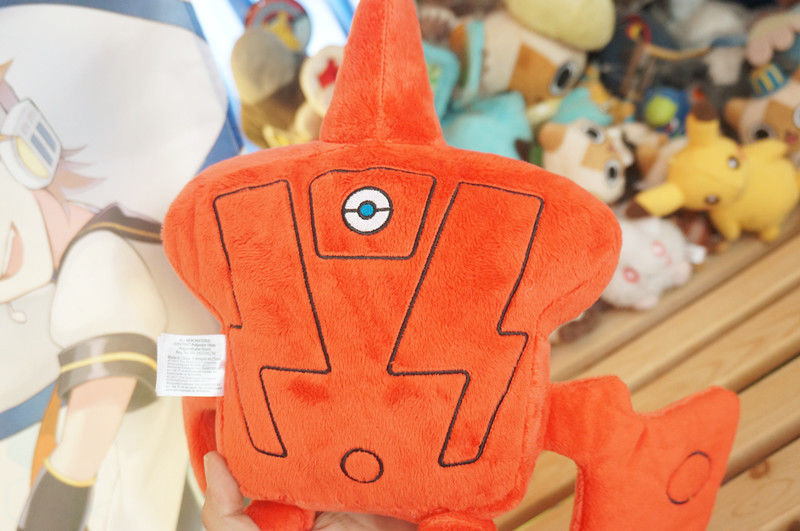
\includegraphics[scale=0.25]{../Images/Back.jpg}
\caption{A visualização do Pokédex. Formato de trás.}
\end{figure}

Pelo projeto inicial, teremos que dividir a idéia em três partes. \newline
- A parte física, o formato do projeto. \newline
- A parte do hardware. \newline
- A parte do software. \newline

O pokédex deve, de modo inicial.: \newline
- Permitir ao usuário de ver todos os pokémons, desde a primeira geração até a geração desse pokédex (Sun and Moon). \newline
- Permitir ao usuário a criar uma equipe de 6 pokémons \newline
- Permitir ao usuário de ver os possíveis items \newline
- Permitir ao usuário a tirar fotos e ver as fotos salvas. \newline

\end{document}